\section{Unmanned Aerial Vehicle}\label{sec:implementation_uav}

The \gls{uav} is the base platform and the main component of the system. For this reason, it is the first component to be implemented. The \gls{uav} is responsible for carrying the reconnaissance platform and the communication system, as well as for executing the flight plan generated by the control station. The detailed implementation of the \gls{uav} is out of the scope of this thesis and only a high-level overview of the implementation is provided. However, more information about the implementation of the \gls{uav} can be found in the \autocite{developingcosteffectivedrones5g}. Each subsystem of the \gls{uav} described in the \cref{sec:design_uav}
is implemented separately and then integrated into the \gls{uav} as a whole.

\subsection{Airframe}\label{subsec:implementation_airframe}

For the airframe, the \gls{uav} was built using following the instructions provided by the manufacturer. The airframe can be seen in \cref{fig:airframe}. However, some modifications were made to the airframe to accommodate the additional components using custom 3D printed parts (e.g., the landing gear, the camera mount, and the payload bay). The design and manufacture of the 3D printed parts where made using the FreeCAD software \autocite{freecadFreeCADYour} and a Bamboo P1S 3D printer \autocite{bambulabBambuPrinter}. The reason to use 3D printed parts is that they are easy to design and manufacture, as well as being lightweight and durable. The 3D printed parts were designed to be easily attached to the airframe using screws and nuts, as well as to be easily removed in case of maintenance or replacement. Some of the 3D printed parts used in the airframe can be seen in \cref{fig:3d_printed_landing_gear_stl}.

\begin{figure}
  \begin{subfigure}{0.4\textwidth}
    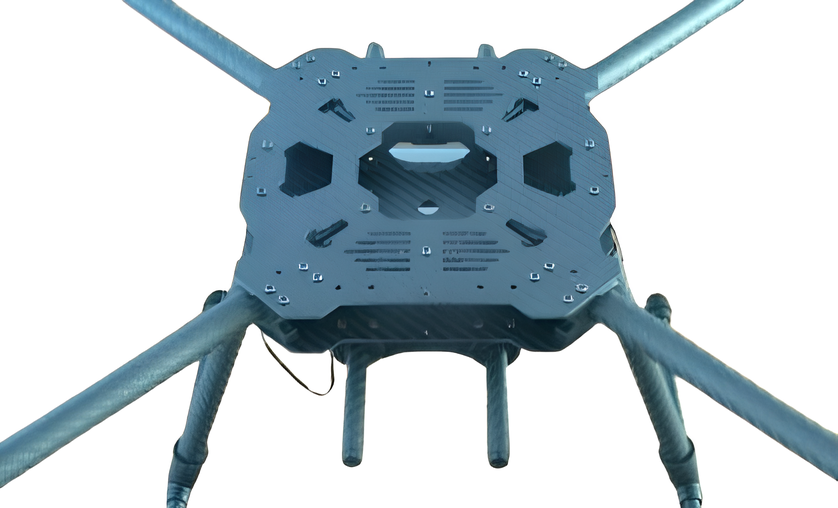
\includegraphics{airframe_tarot.png}
    \caption{Tarot XS690 airframe \autocite{developingcosteffectivedrones5g}.}\label{fig:airframe}
  \end{subfigure}
  \hfill
  \begin{subfigure}{0.4\textwidth}
    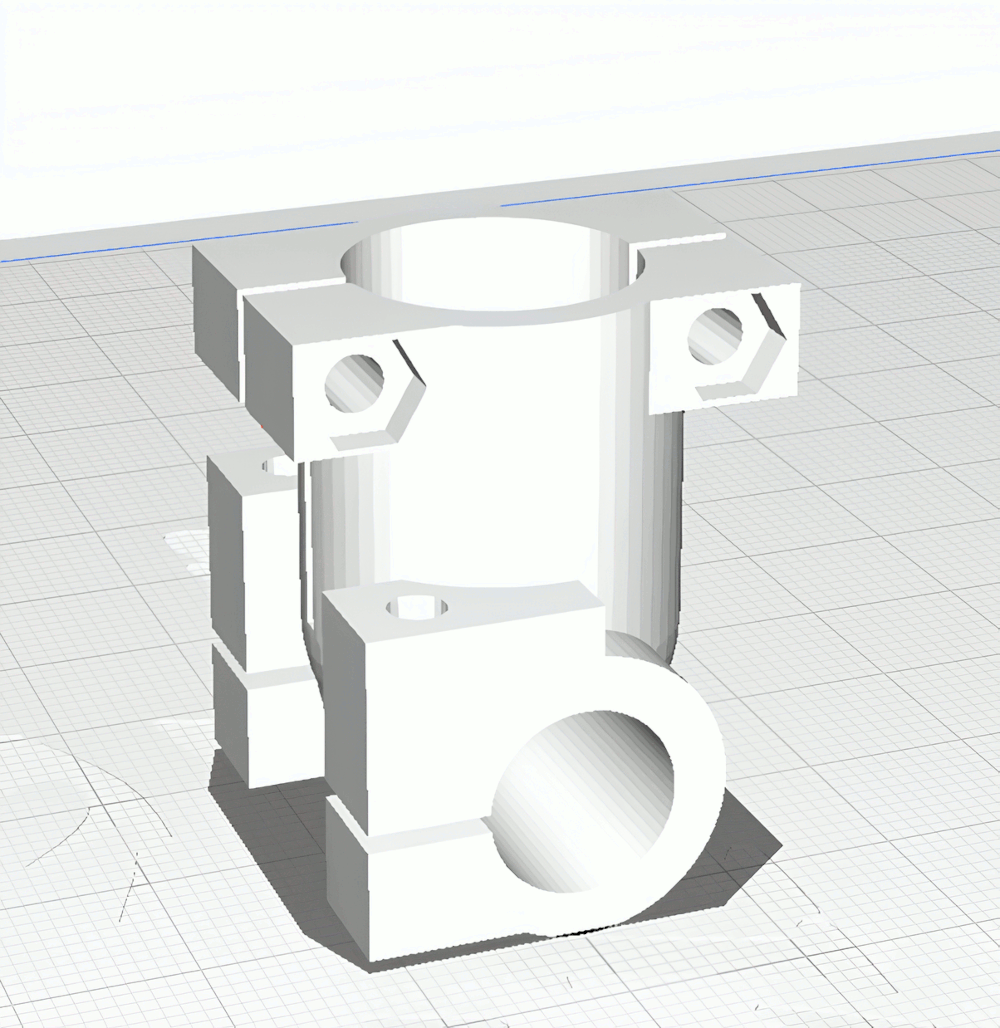
\includegraphics{3d_printed_landing_gear_stl.png}
    \caption{3D printed landing gear \autocite{developingcosteffectivedrones5g}.}\label{fig:3d_printed_landing_gear_stl}
  \end{subfigure}

  \caption{Airframe and 3D printed parts.}\label{fig:airframe_and_3d_printed_parts}
\end{figure}

\subsection{Propulsion System}\label{subsec:implementation_propulsion_system}

Regarding the propulsion system, the four motors were attached to the airframe using custom metal brackets, as seen in \cref{fig:motors_attached_to_airframe}. The \glspl{esc} were attached to the airframe using double-sided tape and zip ties, as seen in \cref{fig:esc_attached_to_airframe}.

\begin{figure}
  \hfill
  \begin{subfigure}{0.4\textwidth}
    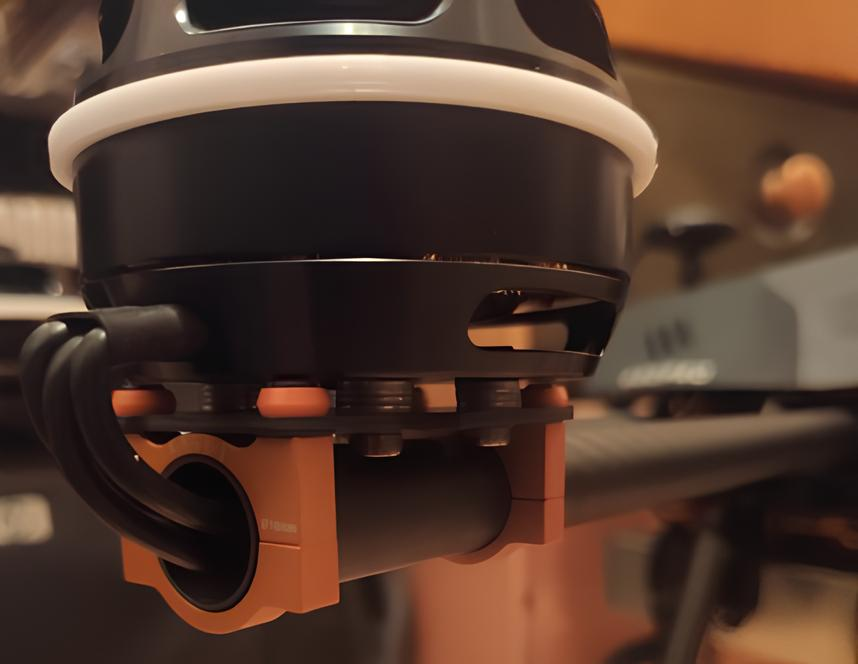
\includegraphics{motor_mount.jpg}
    \caption{Metal motor mount brackets to attach the motors to the airframe (orange brackets) \autocite{developingcosteffectivedrones5g}.}\label{fig:motors_attached_to_airframe}
  \end{subfigure}
  \hfill
  \begin{subfigure}{0.4\textwidth}
    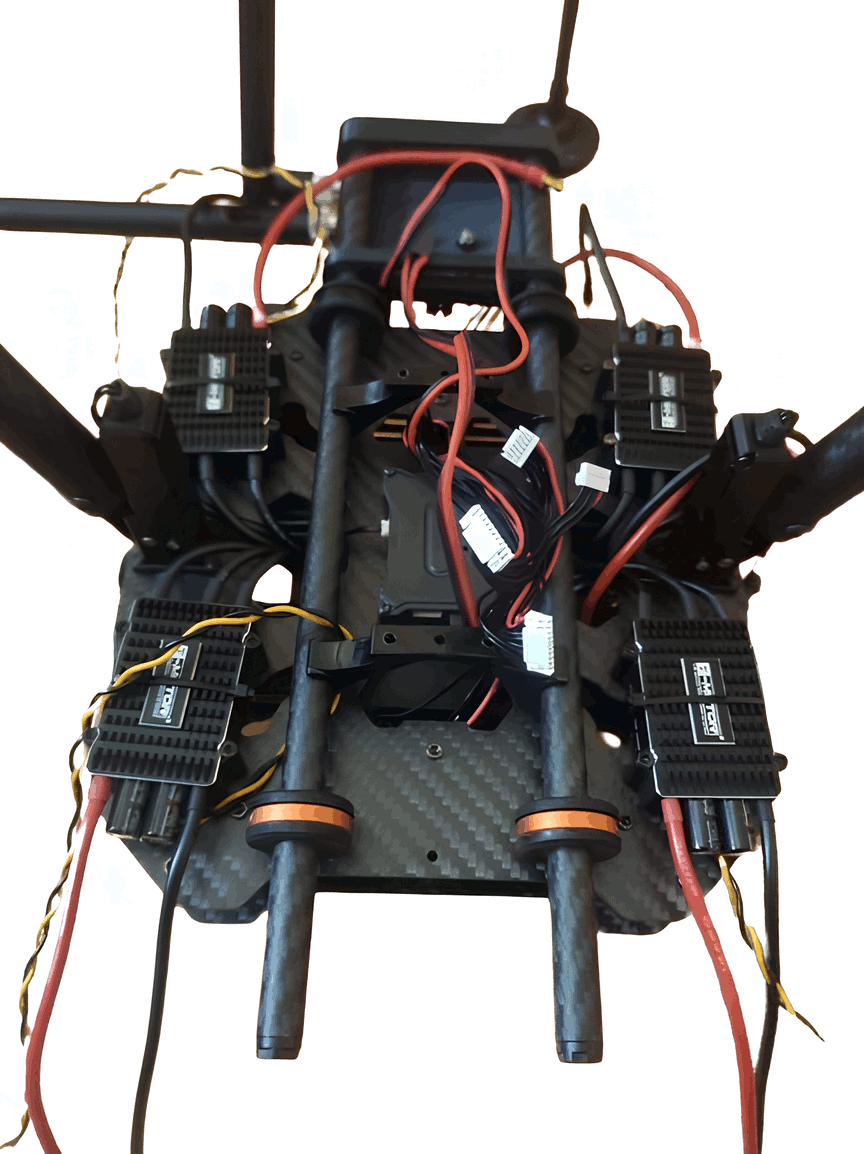
\includegraphics{bottom_plate_esc.png}
    \caption{Bottom view of the airframe with the \glspl{esc} attached in each corner \autocite{developingcosteffectivedrones5g}.}\label{fig:esc_attached_to_airframe}
  \end{subfigure}
  \hfill

  \caption{Propulsion system components attached to the airframe.}\label{fig:propulsion_system_components_attached_to_airframe}
\end{figure}

\subsection{Flight Controller}\label{subsec:implementation_flight_controller}

For the flight controller, it was placed in the middle of the airframe using double-sided tape and zip ties, as seen in \cref{fig:flight_controller_attached_to_airframe}. It is important to note that placing the flight controller in the middle of the airframe provides the best balance and stability for the \gls{uav} during flight.

\begin{figure}
  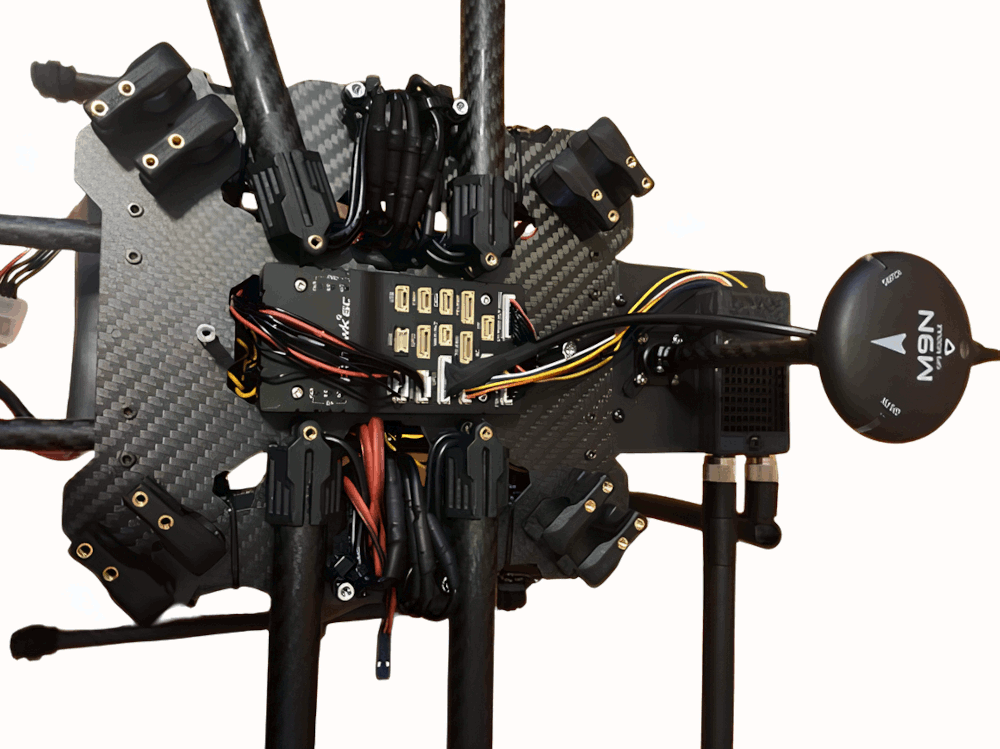
\includegraphics[width=0.4\textwidth]{mid_plate_flight_controller.png}
  \caption{Flight controller attached to the airframe in the middle of the airframe \autocite{developingcosteffectivedrones5g}.}\label{fig:flight_controller_attached_to_airframe}
\end{figure}

\subsection{Power System}\label{subsec:implementation_power_system}

The power system is the heaviest subsystem of the \gls{uav} and must be placed in the center of the airframe to provide the best balance and stability during flight. The battery was attached to the airframe using battery straps, as seen in \cref{fig:battery_attached_to_airframe}. The \gls{pdb}, \cref{fig:pdb}, was attached to the airframe using a custom 3D printed mount and places in the middle of the airframe, as seen in \cref{fig:power_distribution_board_attached_to_airframe}. Also, the voltage regulator was attached to the top of the airframe using double-sided tape and zip ties, refer to \cref{fig:computer_attached_to_airframe}.

\begin{figure}
  \hfill
  \begin{subfigure}[t]{0.3\linewidth}
    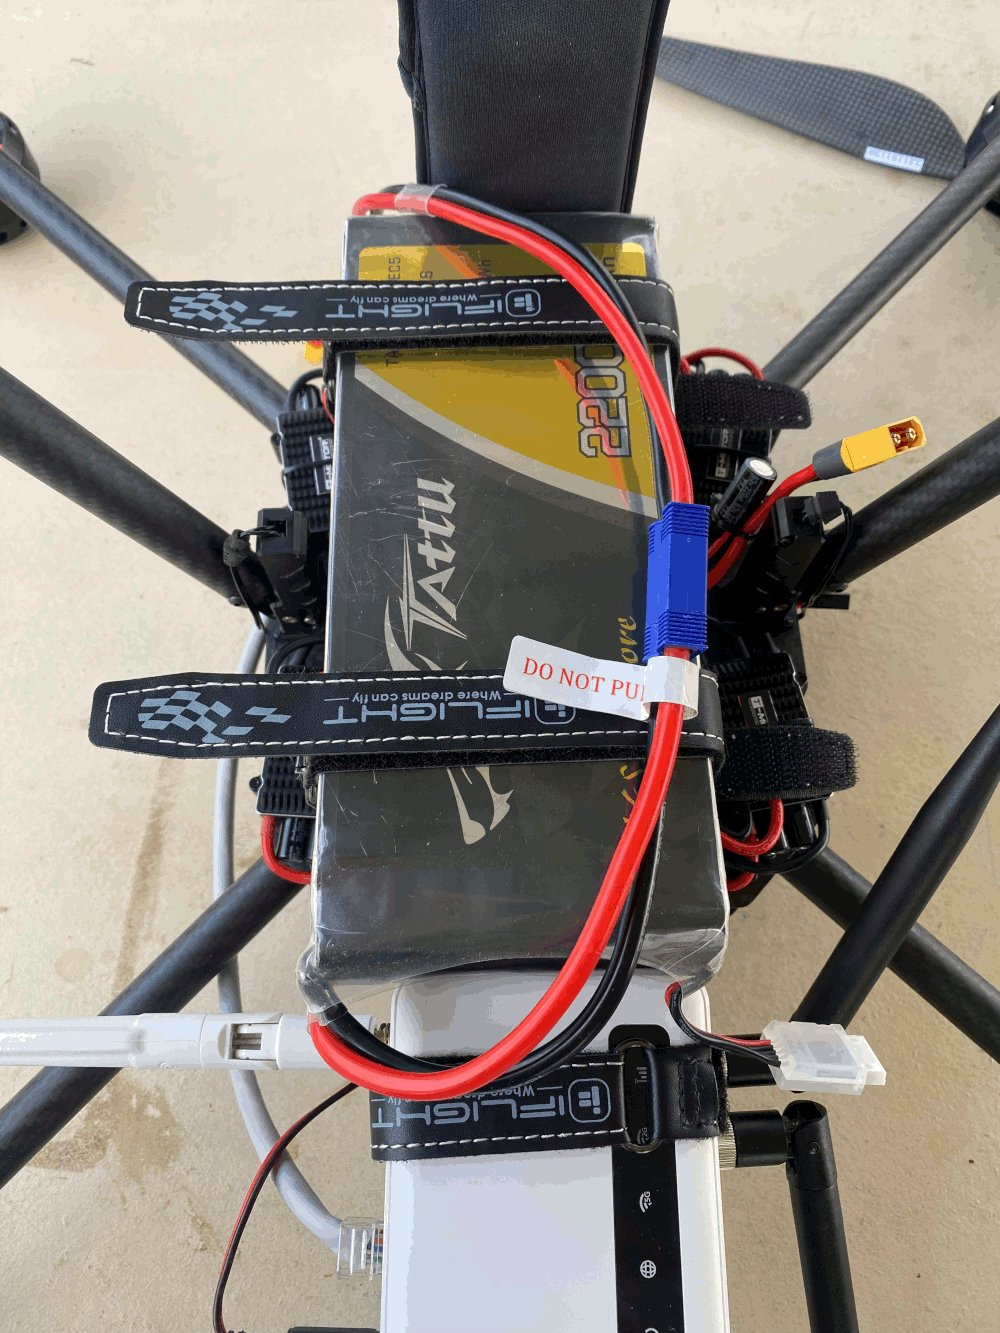
\includegraphics[width=\linewidth]{bottom_plate_battery.jpg}
    \caption{Battery attached to the airframe.}\label{fig:battery_attached_to_airframe}
  \end{subfigure}
  \hfill
  \begin{subfigure}[t]{0.3\linewidth}
    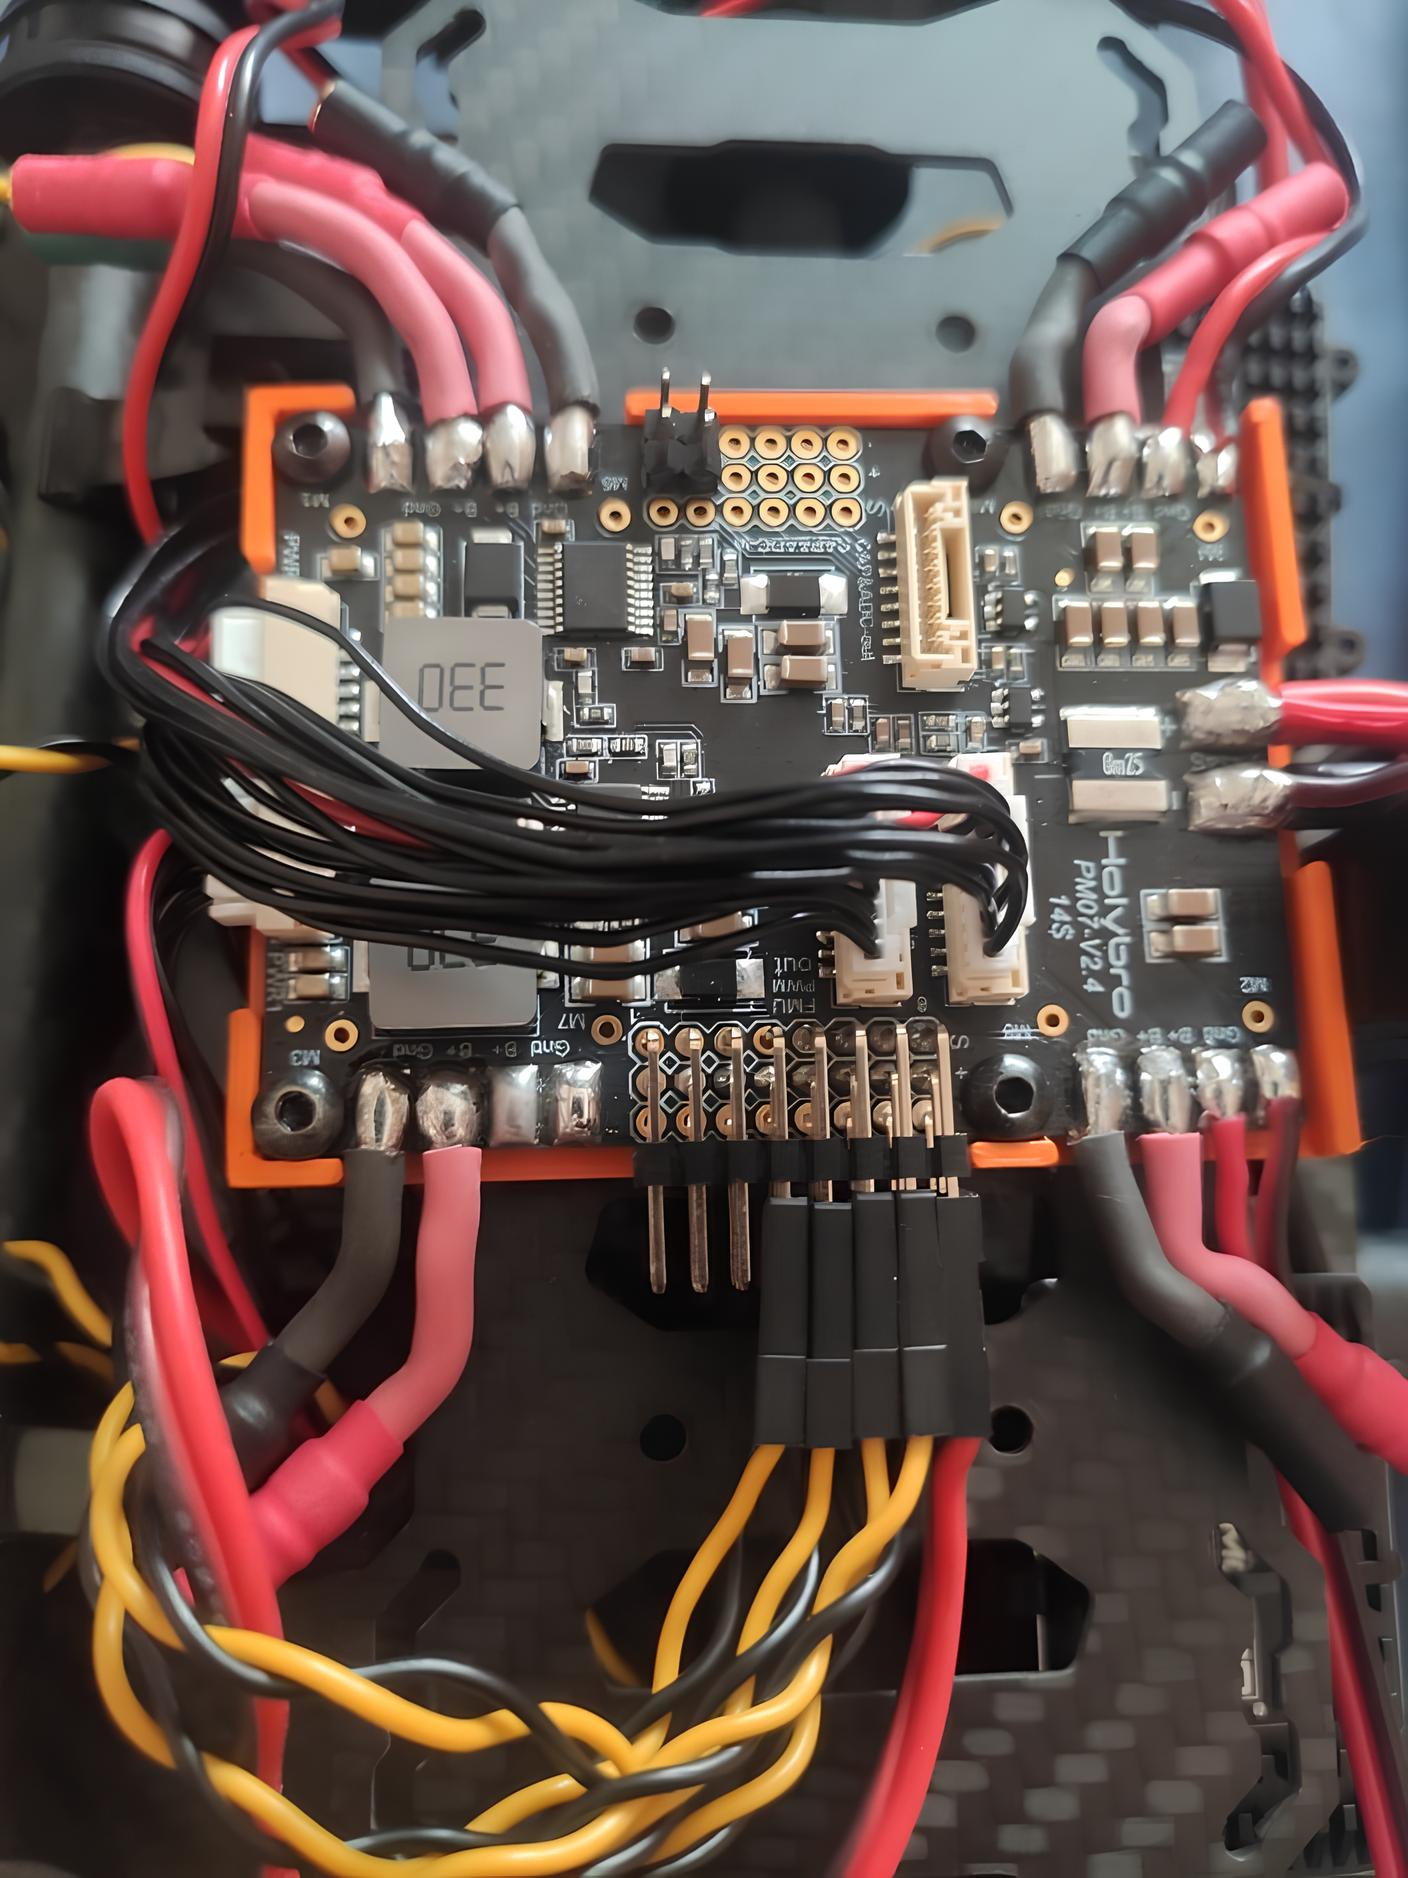
\includegraphics[width=\linewidth]{mid_plate_pdb.jpg}
    \caption{\gls{pdb} attached to the mid plate of the airframe \autocite{developingcosteffectivedrones5g}.}\label{fig:pdb}
  \end{subfigure}
  \hfill
  \begin{subfigure}[t]{0.3\linewidth}
    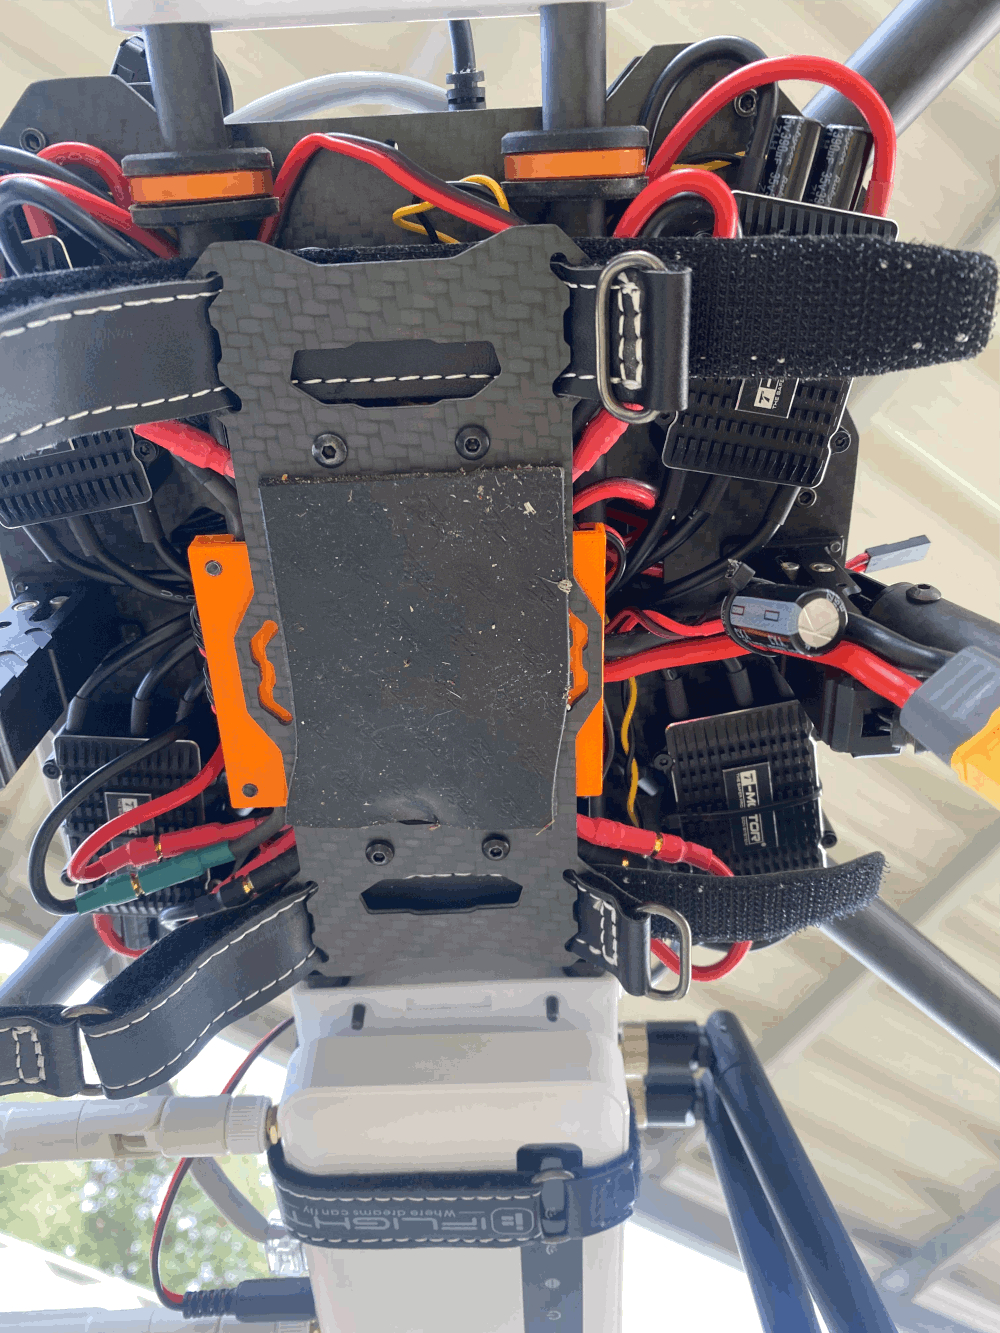
\includegraphics[width=\linewidth]{mid_plate_pdb_mounted.jpg}
    \caption{\gls{pdb} attached to the airframe, orange box in the middle of the airframe.}\label{fig:power_distribution_board_attached_to_airframe}
  \end{subfigure}
  \hfill

  \caption{Power system components attached to the airframe.}\label{fig:power_system_components_attached_to_airframe}
\end{figure}

\subsection{Peripherals}\label{subsec:implementation_peripherals}

The \gls{gps} was attached to the top of the airframe using a custom 3D printed mount, as seen in \cref{fig:gps_attached_to_airframe}. A important note is that the \gls{gps} module must be placed in a location where it has the best reception, as well as where it is not obstructed by other components of the \gls{uav}. It must be place as far as possible from the motors and any carbon fiber components, as they can interfere with the reception of the \gls{gps} module.

For the communication system, the \gls{rf} module was attached to the airframe using the same 3D printed mount as the \gls{gps} module, as seen in \cref{fig:gps_attached_to_airframe}. The \gls{4g} module was attached to the airframe along with the \gls{rf} module and the \gls{gps} module.

The camera was attached to the front of the airframe using a custom 3D printed mount in order to provide the best \gls{fov}, as seen in \cref{fig:camera_attached_to_airframe}. The camera must be placed in a location where it has the best field of view, as well as where it is not obstructed by other components of the \gls{uav}. It must be placed as far as possible from the motors as they can interfere with the camera's \gls{fov}.

Finally, for the on-board computer, it was placed in the middle of the airframe using screws and nuts, as seen in \cref{fig:computer_attached_to_airframe}. It must be placed in a location where air can flow freely to avoid overheating. Depending on the application, the on-board computer can be placed in a different location, as long as it is not obstructed by other components of the \gls{uav}, however, it is recommended to place it in the middle of the airframe to provide the best balance and stability during flight.

\begin{figure}
  \hfill
  \begin{subfigure}[t]{0.3\linewidth}
    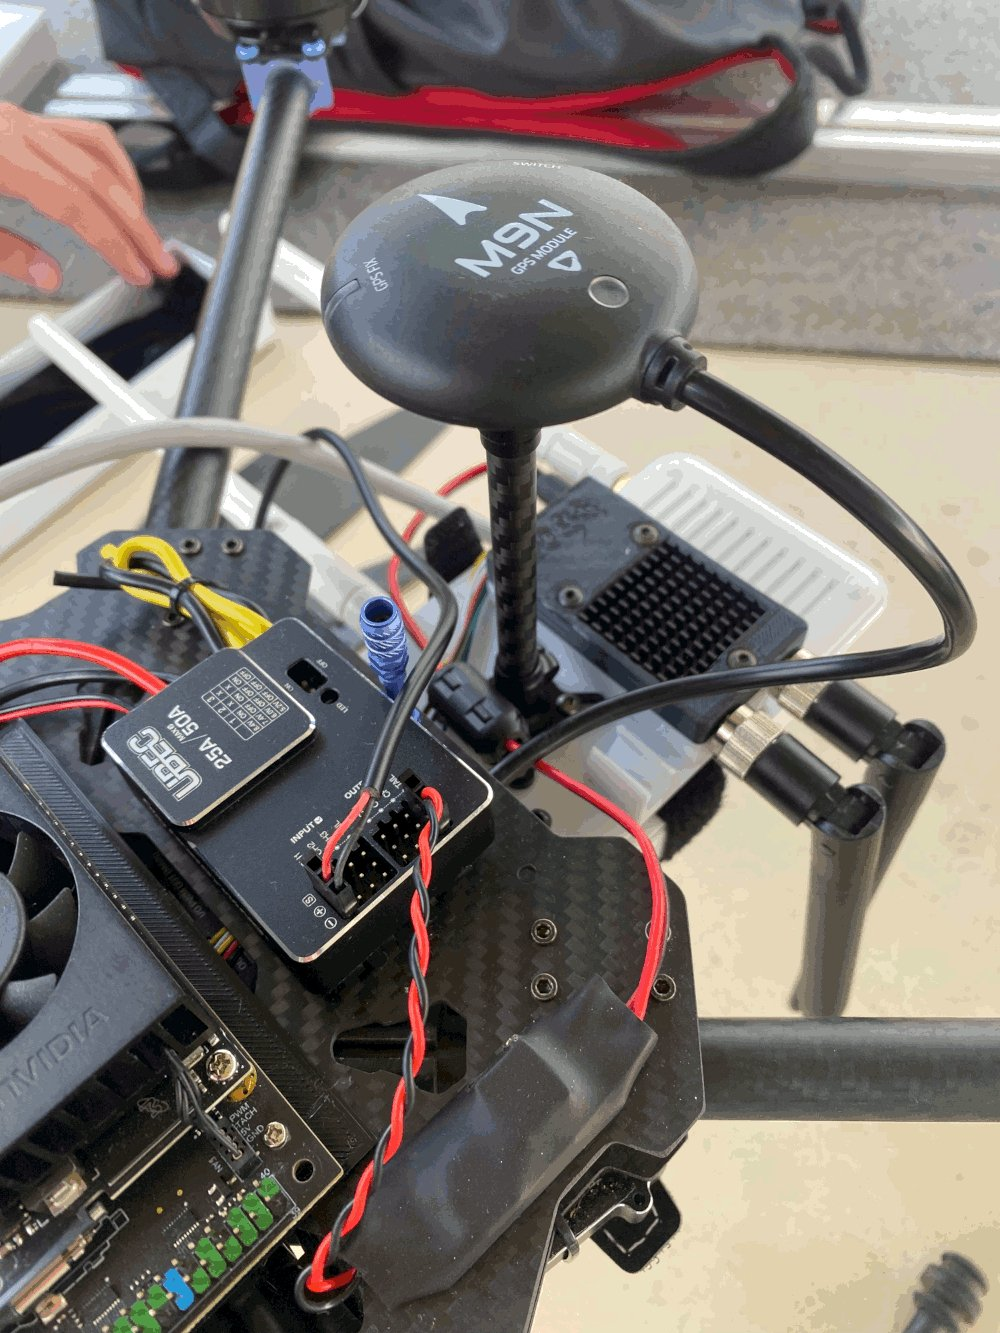
\includegraphics[width=\linewidth]{top_plate_gps.jpg}
    \caption{\gls{gps} module attached to the airframe (circular black module). The \gls{rf} module is the rectangular black module with two antennas behind the \gls{gps} module. The \gls{4g} router is the white module below the \gls{rf} module.}\label{fig:gps_attached_to_airframe}
  \end{subfigure}
  \hfill
  \begin{subfigure}[t]{0.3\linewidth}
    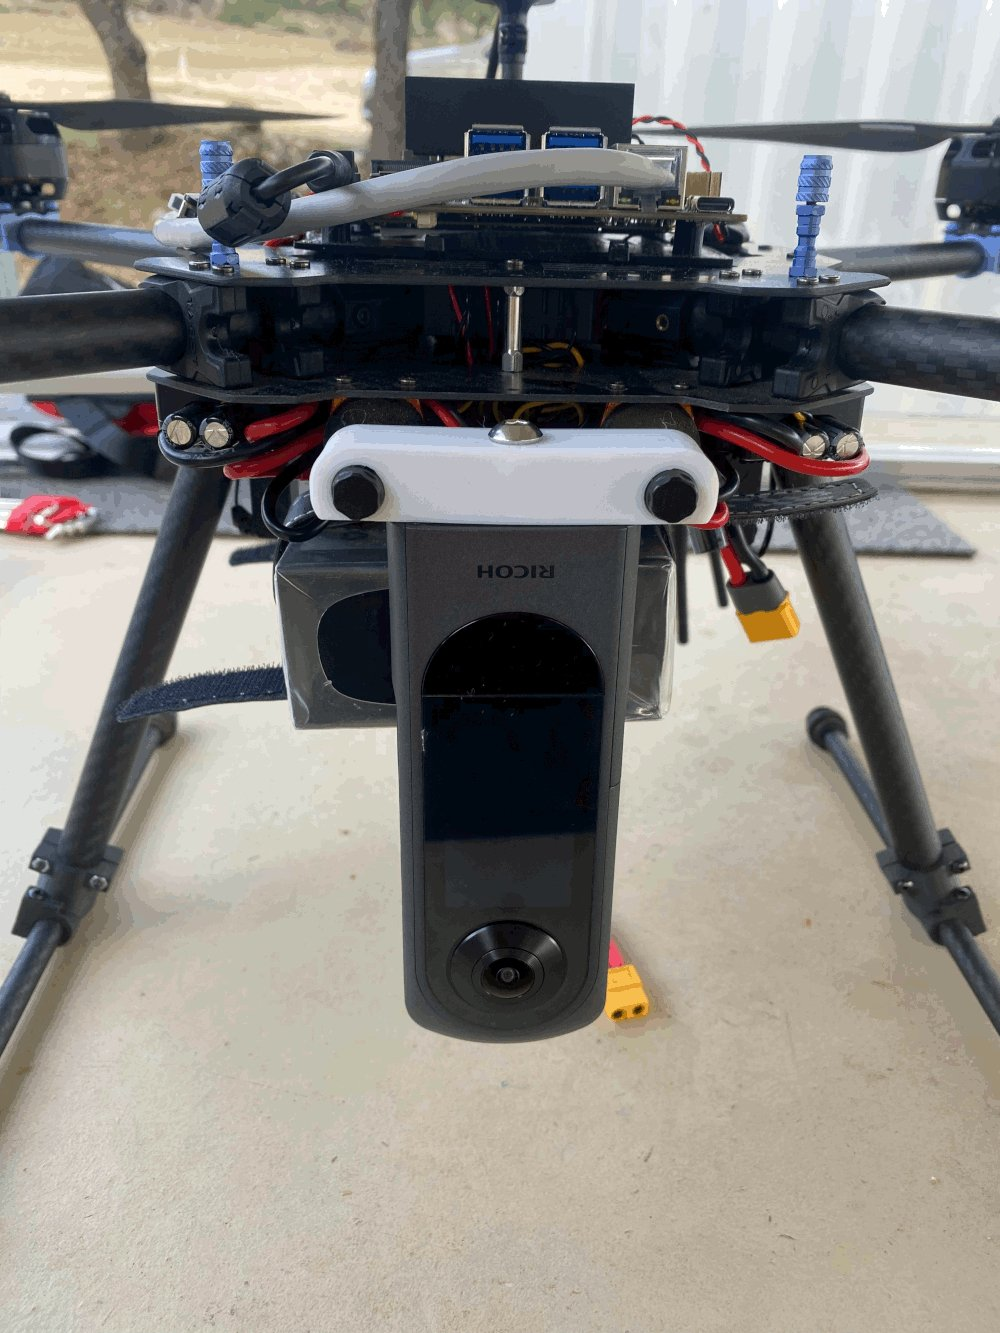
\includegraphics[width=\linewidth]{front_mount_camera.jpg}
    \caption{Camera attached to the airframe using a custom 3D printed white mount.}\label{fig:camera_attached_to_airframe}
  \end{subfigure}
  \hfill
  \begin{subfigure}[t]{0.3\linewidth}
    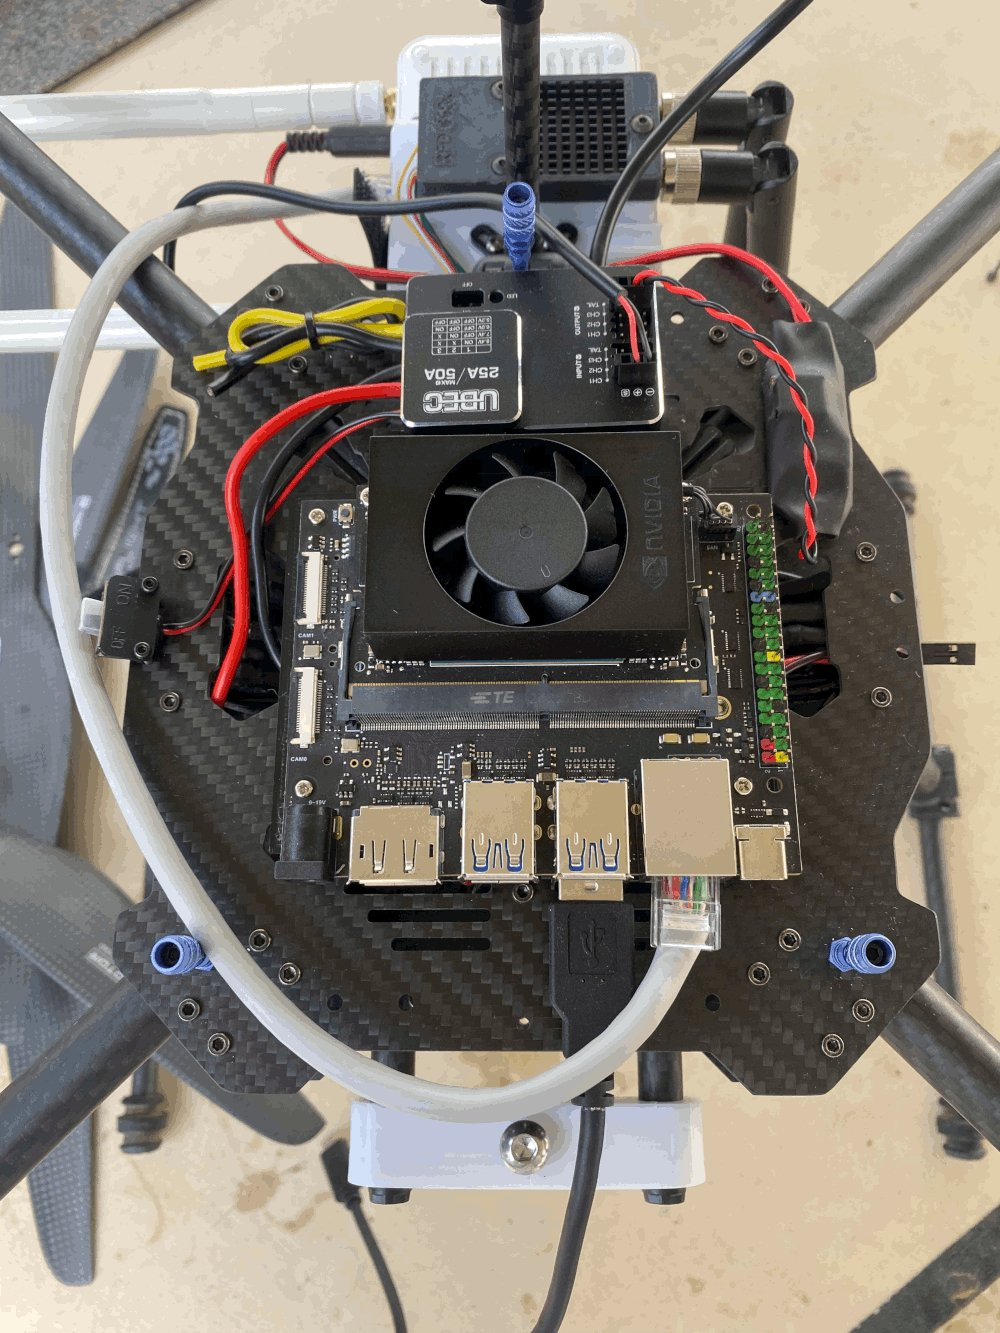
\includegraphics[width=\linewidth]{top_mount_computer.jpg}
    \caption{On the center, the on-board computer. On the top side above the fan, the \gls{gps} module.}\label{fig:computer_attached_to_airframe}
  \end{subfigure}
  \hfill

  \caption{Peripherals attached to the airframe.}\label{fig:peripherals_attached_to_airframe}
\end{figure}

\subsection{Final Assembly}\label{subsec:implementation_final_assembly}

After all the components were attached to the airframe, the final assembly of the \gls{uav} was performed. The final assembly consists of connecting all the components together, as well as configuring the flight controller and the communication system. The final assembly of the \gls{uav} can be seen in \cref{fig:uav_assembled}.

\begin{figure}
  \hfill
  \begin{subfigure}[t]{0.4\linewidth}
    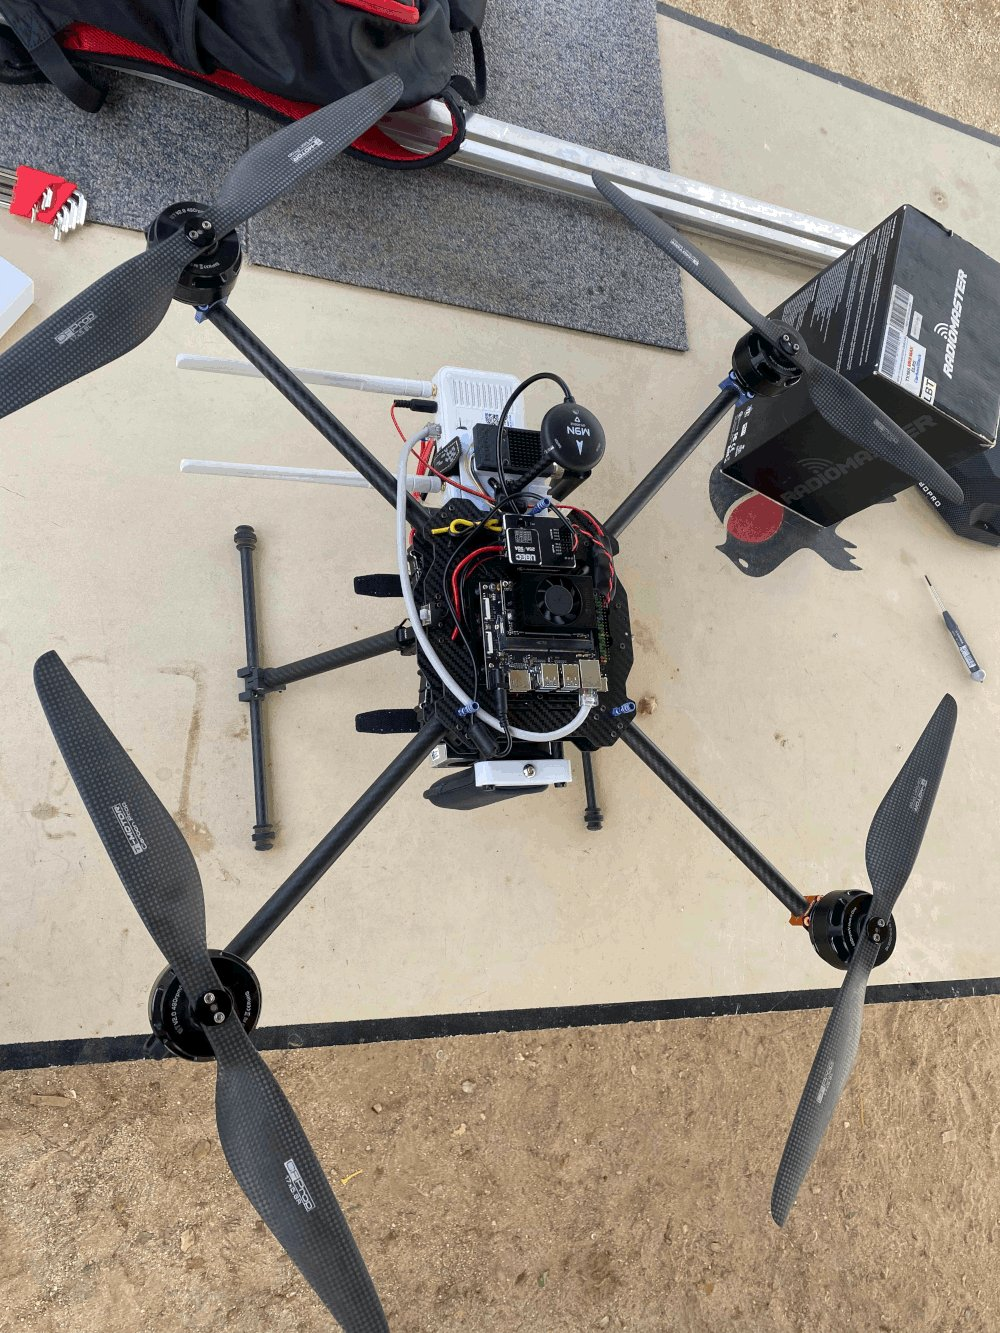
\includegraphics[width=\linewidth]{final_assembly_top.jpg}
    \caption{Top view of the \gls{uav} assembled.}\label{fig:uav_assembled_top}
  \end{subfigure}
  \hfill
  \begin{subfigure}[t]{0.4\linewidth}
    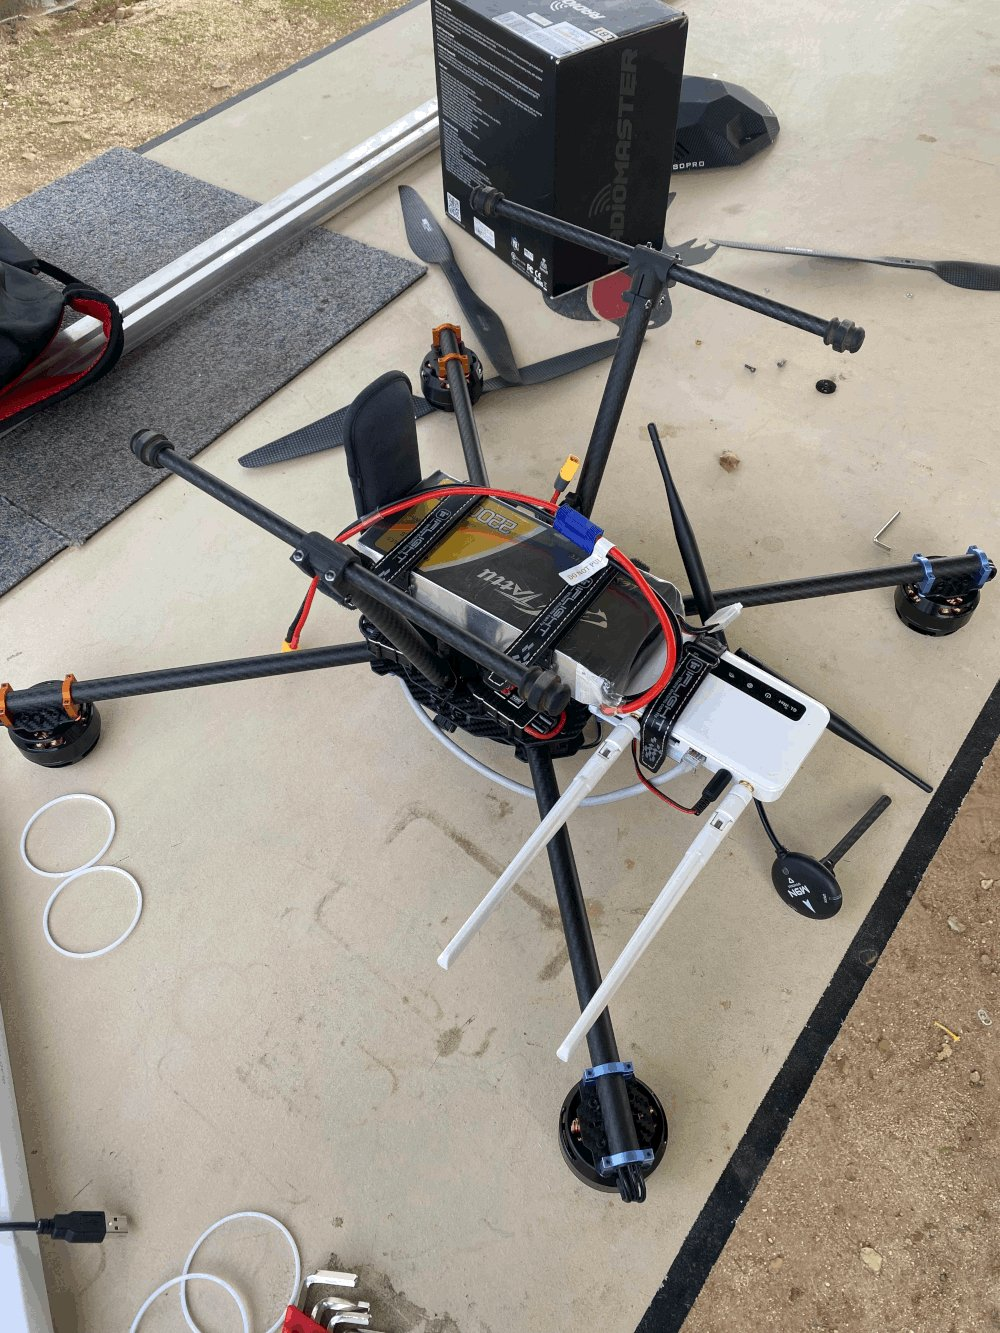
\includegraphics[width=\linewidth]{final_assembly_bottom.jpg}
    \caption{Bottom view of the \gls{uav} assembled.}\label{fig:uav_assembled_bottom}
  \end{subfigure}
  \hfill

  \caption{Final assembly of the \gls{uav}.}\label{fig:uav_assembled}
\end{figure}
